\section{System Design} 
\animatedead{} incorporates a PHP emulator which is capable of emulating the execution of PHP code in an environment with abstract entities (e.g., user-provided values, database, network, etc.). 
Figure~\ref{fig:ad_diagram} shows an overview of our system. 
We start by discussing the process to collect the web application entry points. 
Next, we review the design of our emulator and its distributed analysis scheme. 
Then we go over the challenges of PHP symbolic execution such as state space explosion and discuss our approach to addressing them. 
Finally, we use the code-coverage produced by concolic execution of target web applications to perform a module reachability analysis and debloat unused files and functions. 

\begin{figure}[t]
	\centering
	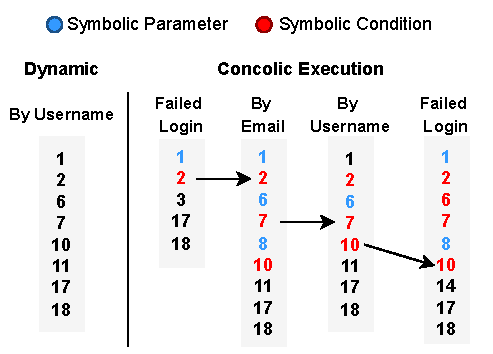
\includegraphics[width=0.5\linewidth]{figures/ad/code_sample_concolic.pdf}
	\caption{Dynamic code-coverage of a successful login attempt vs. symbolic execution of the same entry point. In this sample, user-provided parameters (e.g., \texttt{\$\_POST[\textquotesingle{}user\textquotesingle{}]}) and database operations (e.g., \texttt{get\_user\_by()}) are symbolic. Arrows mark the exploration of new feasible branches as determined by the symbolic engine.}
	\label{fig:concolic_coverage}
\end{figure}

\begin{figure*}[t]
    \centering
    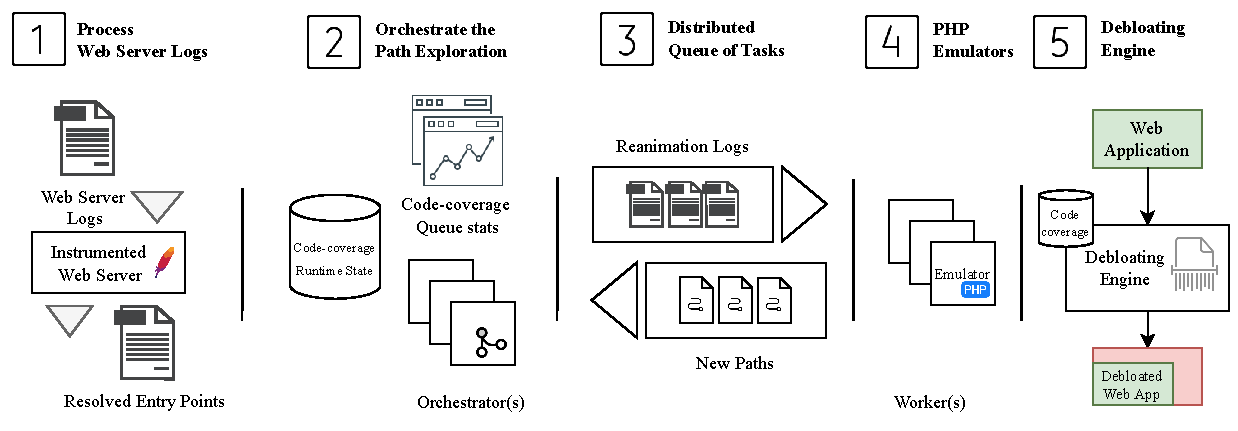
\includegraphics[width=\textwidth]{figures/ad/animatedead_diagram.pdf}
    \caption{Overview of Distributed \animatedead{}. In Stage 1, \animatedead{} analyzes the web server log files to generate unique web application entry points. Orchestrator nodes and workers (Stage 2 and 4) interact over message queues (Stage 3) to identify which paths should be explored by the emulators, \animatedead{} provides a realtime reporting panel that plots the size of the queue and newly identified code-coverage over time. Finally, in Stage 5, the overall code-coverage from concolic execution is incorporated for reachability analysis and unreachable modules from the entry points are debloated. Orchestrators and worker nodes run in container environments and can be scaled up on demand.}
    \label{fig:ad_diagram}
    \vspace{-1em}
\end{figure*}

\subsection{Application Entry Points}
The first step of our analysis consists of collection and processing of web application entry points.  
By using the existing logging mechanism of web servers, \animatedead{} is able to analyze web applications with \emph{no} extra runtime performance overhead. 
At the end of this stage (Step 1 in Figure~\ref{fig:ad_diagram}), we provide the list of PHP scripts and their concrete (e.g., GET parameters) and symbolic parameters (e.g., POST parameters, file uploads, cookies, etc.) to \animatedead{}'s PHP emulators for concolic execution. 

\subsubsection*{Analyzing Web Server Log Files} 
After collecting the web server logs for the target web application, \animatedead{} merges and de-duplicates the entries. 
The level of information provided for each entry point (i.e., concrete inputs) has a direct effect on the time of analysis. 
By shrinking the state space of the analysis via providing more detailed logs, we can reduce the total number of paths and reduce the overall analysis time. 

To that end, we experimented with the default fields of information in web server logs and extended logs. 
To generate extended logs, we use the web server's configuration options to include high level information such as the name (but not the value) of cookies, POST parameters and the file uploads. 
The extra information included in the extended logs limits the concolic execution to only explore paths that rely on the parameters that we have seen previously in the logs. 
Extended logs are particularly helpful for larger web applications such as WordPress and phpMyAdmin where a single entry point is responsible for a diverse list of features depending on the provided parameters. 
For instance, phpMyAdmin uses the same \emph{index.php} entry point combined with the \emph{target} GET parameter to generate the content of the requested pages. 
Providing this parameter to \animatedead{} allows it to only explore code-paths for the desired feature. 

\subsubsection*{Analyzing Log Files With URL Rewriting} 
PHP applications commonly incorporate URL rewriting to provide a user-friendly experience to their visitors and improve the search engine optimization of their website. 
Through this step, the original requested URIs are translated to one of the web application entry points either by the web server (e.g., Apache rewrite module and \texttt{.htaccess} files) or an internal module within the web application (i.e., custom routing modules). 
In the latter case, our PHP emulator resolves this mapping automatically without requiring any further action. 

For web applications using the web server's rewriting feature, the web server transforms the URIs before passing them to the web application. 
For such web applications, \animatedead{} dynamically replays the requests towards its integrated instrumented web server hosting a copy of target web applications and returns the translated entry points. 

\animatedead{} includes an instrumented Apache web server in its docker environment that hooks into every request and returns the translated URIs. 
By intercepting the incoming requests, \animatedead{} takes control of the execution and returns the resolved entry point after the web server applies the rewriting rules.
% Using PHP's \texttt{auto\_prepend\_file} directive, \animatedead{} takes control of the execution while the web server acts upon the original rewriting rules from the source code of target web applications under analysis. 
% This option can be enabled through \animatedead{}'s configuration file. 

\subsection{PHP Emulator}
Concolic execution requires a modified PHP execution environment that can operate based on symbolic parameters. 
We developed a PHP emulator for \animatedead{} that closely represents the PHP engine itself and operates based on the source code of PHP scripts. 
The analysis for each PHP application starts by parsing each entry point (e.g., \emph{index.php}) into it's respective Abstract Syntax Tree (AST) and traversing it. 
Through this traversal, certain PHP instructions will expand the AST during emulation. 
File inclusions, class instantiations, function calls and dynamic code generation routines (e.g., \texttt{eval}) can add new nodes to the AST. 

\animatedead{}'s emulator executes the PHP instructions of the program under analysis and resolves the dynamic code structures to generate a complete AST. 
In practice, resolution of dynamic code structures requires the precise implementation of every language construct and modeling its effects on the state of the emulator (i.e., active namespaces, current object pointers, variable scopes, function calls and return values, etc.). 

In \animatedead{}, beyond modeling the 188 standard PHP opcodes~\cite{popov}, we model the built-in PHP functions that affect the state of the emulator (e.g., loading new classes and defining new constants). 
For the majority of the self-contained PHP built-in functions that do not change the state of the emulator or manipulate the flow of execution such as \texttt{date}, \texttt{print}, \texttt{explode}, \texttt{file\_exists}, etc. we first resolve their arguments and then, invoke the original implementation in the PHP engine. 
For functions that rely on the state of the emulator (e.g., \texttt{class\_exists}, \texttt{define} (defines a new constant), \texttt{reflection APIs} (rely on autoloader and loaded classes and can invoke new code), \texttt{eval}, etc.), we provide our own implementation in the emulator. 
After a careful review of PHP documents and the list of built-in functions used in popular PHP applications, we identified 92 functions that required a custom implementation in our emulator. 

\animatedead{}'s PHP emulator is written in PHP 7.4 and is capable of emulating PHP 5.x and 7.x. 
The emulator imports all the environment variables and predefined constants (e.g., PHP version, default include path, etc.) from an existing web server environment. 
Moreover, analysts using \animatedead{} can override any desired API through the provided configuration file. 

We built our PHP emulator by extending the emulator developed by Naderi et al. called MalMax, which the authors combined with counterfactual execution to uncover the hidden behavior of obfuscated PHP malware~\cite{naderi2019malmax}. 
MalMax was originally built for PHP 5, and did not support symbolic execution. 
We spent over 13 person/months developing and testing our PHP emulator that supports the PHP language features used by popular PHP applications. 

One of our main contributions to MalMax's emulator is the distributed symbolic execution engine. 
Moreover, we added support for integral features of the PHP language to our emulator including the new PHP 7 instructions, object orientation features (e.g., inheritance, interfaces, etc.), closures, anonymous functions, namespaces, and reflection. 
Through this effort, we have doubled the code size of the original PHP emulator of MalMax, and the final \animatedead{} (i.e., emulator plus distributed execution environment) is more than five times the size of the initial emulator. 

\subsection{Handling Symbolic Operations and Logic}
\animatedead{} uses a configurable list of symbolic inputs (i.e., user-provided variables and system APIs). 
In this section, we explain the design details of our concolic emulator, including the type tracking, value set analysis, and the transition from symbolic to concrete values. 



\subsubsection{Concolic Execution}
\label{sec:concolic_translation}
One of the main requirements of a symbolic execution engine is to continue the program's execution with an abstract state of variables. 
At a high level, when dealing with symbolic program variables, PHP instructions such as conditionals would need to explore all the feasible branches when provided with a symbolic condition. 
Similarly, assignment instructions propagate the symbolic values upon their execution.

Our emulator incorporates type tracking to extract the type of symbolic variables even when the actual value is unknown. 
The variable type information is then used to skip the exploration of unsatisfiable branches. 
We model built-in functions that rely on variable types (e.g., \texttt{is\_int}) in the emulator for an accurate execution. 
Similarly, we include our own implementation for instructions that dynamically add new nodes to the AST (i.e., dynamic file inclusion, dynamic function calls, and dynamic object instantiation). 
More specifically, \animatedead{} uses the information available through the execution environment to transform the symbolic variables to their concolic equivalents. 
We will discuss this in more detail later in this section.

An example of this transition is reflected in file export format selection in phpMyAdmin which includes options such as SQL, CSV, Zip, etc. 
Given a symbolic export type in the form of user-controlled variable, \animatedead{} cannot statically determine which of the underlying export plugins should be loaded. 
The \texttt{Plugin\_loader} module within phpMyAdmin performs a series of string operations to sanitize the user input and to transform the selected export format to one of the available plugins on the file-system under the \texttt{libraries/plugins/export/} directory. 
As a result, by following the conditions enforced on the export format variable through execution (e.g., fixed prefix, file extension, and allow-list membership checks), \animatedead{}'s emulator can accurately identify the list of available export plugins in phpMyAdmin. 
Then, the emulator will explore the execution of the underlying entry point using each individual export plugin. 

\paragraph{Type tracking and value set analysis:} 
We have augmented our PHP emulator to track the type of symbolic variables based on known return type of PHP instructions and APIs. 
For instance, casting a symbolic variable to a specific type or invoking built-in functions with known return types (e.g., \texttt{substr} $\rightarrow$ \texttt{string}, or \texttt{isset} $\rightarrow$ \texttt{boolean}) will determine the resulting type of that variable. 
Unfortunately the information about the type of return values from PHP built-in functions is not available through the PHP reflection API. 
Instead, we extracted this information from the PHP documentation and incorporated it in \animatedead{}. 

Moreover, we model regex and string operations (e.g., \texttt{strncmp(\textquotesingle{}pma\textquotesingle{}, \$cookie\_name, 3) \!= 0}) as part of our emulator. 
By doing so, for path conditions that rely on these operations, we track the constraints applied to the underlying variables. 
This way, \animatedead{} can determine non-feasible conditions and refrain from exploring them. 

Lastly, we perform a scope-specific value set analysis. 
Web applications commonly perform allow-list and block-list checks to sanitize user-provided parameters and database sourced values. 
For instance, phpMyAdmin performs the following allow-list check to sanitize and validate the user-provided viewing mode in the reporting tabs: \texttt{in\_array(\$\_REQUEST[\textquotesingle{}viewing\_mode\textquotesingle{}], array(\textquotesingle{}server\textquotesingle{}, \textquotesingle{}db\textquotesingle{}, \textquotesingle{}table\textquotesingle{})}. 
When exploring paths that satisfy this symbolic condition, \animatedead{} limits the possible values of the symbolic \texttt{\textquotesingle{}viewing\_mode\textquotesingle{}} parameter to the values in the corresponding array (i.e., \texttt{\textquotesingle{}server\textquotesingle{}}, \texttt{\textquotesingle{}db\textquotesingle{}}, or \texttt{\textquotesingle{}table\textquotesingle{}}). 
This feature helps reduce the total number of explored branches and also aids the concolic engine when transitioning from symbolic values to their concrete counterparts. 


\paragraph{Transition from symbolic to concrete values:} 
The main benefit of symbolic execution is that each symbolic value represents all the possible values for that variable. 
As a result, it is beneficial to continue the execution with symbolic values. 
However, there exists scenarios in which \animatedead{} cannot continue executing the target application symbolically. 

Whenever our emulator reaches a PHP instruction that can change the structure of the AST by adding new files or calling new functions, \animatedead{} must replace the symbolic inputs of that API with its concrete counterparts. 
Examples of the APIs that add new nodes to the AST are file inclusion APIs (e.g., \texttt{include \$var}), class instantiations and static function calls that trigger the PHP autoloader (e.g., \texttt{new \$var} or \texttt{\$var::static\_function()}), reflection APIs, variable function calls (\texttt{\$var()}), APIs accepting a callback (e.g., \texttt{call\_user\_func(\$var)} and \texttt{preg\_replace\_callback(/regex/, \$var)}). 

In any of the aforementioned cases, \animatedead{} will rely on the information available from the execution environment to transition to concrete values. 
Most commonly, this step would consist of using the type information to determine the class type (for object instantiation), mapping the string operations to the file system or using the information from the value set analysis to determine the candidate values for each symbolic variable. 

Whenever the emulator faces more than one concrete option for a symbolic variable, it will create a new task including the code-coverage of the current execution and information about the concrete values for the target variable and add this task to the queue for future concolic execution (bottom queue in Step 3 in Figure~\ref{fig:ad_diagram}). 
Orchestrators process the code-coverage of each execution. 
Discovery of new code-coverage increases the priority of descendant paths of the current execution. 
\animatedead{} provides a configuration option to limit the total number of concrete values added from each point in the web application. 
% Based on our observations on PHP applications and their coding patterns, we set this limit to 20. 

In the scenario where symbolic execution cannot provide any information about the value of variables used in dynamic file inclusions or function calls, \animatedead{} would not be able to correctly determine the target files and functions to execute next. 
While in theory such code structures exist, and they could lead to false positives, in practice, we did not observe \emph{any} of them. 
An unbound symbolic file inclusion or function call may be rooted in non-sanitized user controlled variables or parameters coming from the database. 
In both scenarios, this could signal the presence of a first or second order injection style vulnerability and requires further attention. 
We incorporated safety checks within \animatedead{} to prevent the inclusion of an uncontrollably large number files or functions when the symbolic parameter is unbound and instead, we alert the analysts. 

\subsubsection{Emulation Replay} 

Throughout the analysis of PHP scripts, for every branch with symbolic condition, \animatedead{} explores all feasible paths. 
Similarly, when transitioning from symbolic to concrete values, multiple execution states are added to the queue. 
Upon facing more than one path to explore, the emulator produces a log called ``reanimation log'' which marks the currently explored branches and lists the next symbolic branch that should be explored. 
Using the reanimation logs, \animatedead{} instructs the emulator in worker nodes to replay the same execution and explore new branches within the code (top queue in Step 3 of Figure~\ref{fig:ad_diagram}). 


\subsubsection{Sources of Symbolic Information} 

In our analysis, we marked HTTP requests and their parameters, database APIs, and network APIs as symbolic. 
Therefore, the result of the analysis is a generalization over \emph{all} the possible values for the parameters present in the web server logs for the application under analysis. 
In our study we opted to run our analyses with an abstract application database. 
This way, our analysis generalizes for \emph{all} deployments of the web applications with any state of the database (i.e., successful and failed connections, empty and non-empty tables, etc.). 
Lastly, we mark network request responses as symbolic to account for successful and failed requests (e.g., checking for updates).

For HTTP requests, we instruct \animatedead{} that HTTP Cookies, Session variables, and File upload and POST parameters (For POST requests) are symbolic. 
This is based on the intuition that web servers will log HTTP GET request parameters and their values by default (i.e., URL query strings) but the value of cookies, session variables, and POST parameters are not included in neither default nor extended logs as they can include sensitive information. 
For database abstraction, we referred to the PHP language documents to extract the list of database APIs for popular database backends~\cite{phpdatabaseapis} and marked them as sources of symbolic information. 
Lastly, we marked PHP cURL APIs as symbolic to abstract the effect of network requests. 

\paragraph{Handling file uploads and file modifications/deletions:} 
PHP engine stores information about the uploaded files in the \texttt{\$\_FILES} super global variable. 
Each entry in this array corresponds to one of the user-uploaded files and contains information such as name, mime-type, temporary name (i.e., temporary file storage under /tmp/php/ directory by default), error (error code or 0 if successful), and size (upload size in bytes). 

For entry points with file uploads, \animatedead{} populates this super global variable with symbolic entries including successful and failed file uploads. 
Moreover, file operation APIs (e.g., \texttt{fopen, file\_get\_contents}, etc.) are modeled inside our emulator to handle symbolic file uploads. 
That is, opening a symbolic file will return a file with symbolic content. 
All web applications in our dataset perform file upload operations and our tests invoke the underlying entry points. 

When running multiple concolic execution workers in parallel, we isolate the changes they make to the file system to prevent side effects on other executions. 
\animatedead{} intercepts the APIs used to modify (e.g., \texttt{file\_put\_contents}) or remove files (e.g., \texttt{unlink}) and changes made through these APIs are only visible to the currently running execution. 
Therefore, file system modifications from one worker do not affect future executions and other workers. 

\subsection{Distributed Concolic Execution} 

Throughout the analysis of target applications, \animatedead{} will explore millions of different paths. 
To scale up the analysis, we designed a distributed environment with various worker processes running our PHP emulator. 
In this setup, we designate a group of orchestrator nodes responsible for the code-coverage analysis of the workers and prioritization of next paths to explore (Step 2 in Figure~\ref{fig:ad_diagram}). 
Orchestrators compare the code-coverage of current execution with the previously explored code and prioritize the analysis of unexplored branches, specifically the descendants of executions that resulted in the exploration of new parts of the code-base. 

\subsubsection{Path Prioritization}

We try to address the problem of state space explosion from two directions:
\begin{itemize}
    \item Eliminating unsatisfiable paths and limiting the total number of explored paths.
    \item Prioritizing paths based on their likelihood to explore unique parts of the codebase.
\end{itemize}

\paragraph{Reducing the total number of feasible paths:} 
Through close inspection of the structure of popular web applications, we identified that the majority of symbolic conditions check for presence or absence of user-provided parameters. 
These parameters usually dictate the main control flow of the entry points (e.g., providing username and password in a login request). 

Given the list of user controlled parameters (i.e., Post, Cookie, and Session variables) in phpMyAdmin, we analyzed the constraints for symbolic conditions. 
Overall, we identified that on average, 72\% of symbolic conditions only check for presence or absence of such parameters through the \texttt{isset} and \texttt{empty} built-in functions. 

Based on this observation, we decided to include the name (and not the value) of these parameters in the extended web server logs. 
This way, we will have the list of provided parameters by the users for POST requests and file uploads, thereby, significantly reducing the number of symbolic paths to be explored by \animatedead{}. 
% Moreover, we use the type tracking of \animatedead{} to eliminate the exploration of unsatisfiable branches in conditions on symbolic variables with a known type. 

\paragraph{Efficient path selection:} 
The exponential growth in the total number of paths in the application under analysis requires an effective path selection strategy. 
Symbolic execution engines employ problem-specific heuristics to analyze paths that are more likely to yield the desired results first. 
In the current setup, we opted to optimize paths to maximize code-coverage that is reachable from each entry point. 
\animatedead{} implements two path prioritization algorithms:

\begin{itemize}
    \item \textbf{DFS:} Using the depth-first-search algorithm, emulator worker processes will choose the last symbolic branch and flip its last symbolic condition to explore the new paths. This is the most straightforward approach that lacks any optimization for maximizing the explored code-coverage. 
    This method would result in the assignment of the same priority to all paths.
    \item \textbf{Branch-coverage guided prioritization:} In this setup, orchestrator nodes keep track of the branch coverage across all workers and prioritize paths that will explore the unseen branches. 
    For branches that have never been explored before, we set the priority to the maximum of 100. 
    After covering all the unique branches at least once, we calculate the priority by adding the total number of new lines discovered by each execution to 20\% of the priority of the parent branch for a maximum of 100. 
    This way, we focus on expanding the coverage in the vicinity of the recently discovered code, while gradually reducing the effect of the priority inherited from the parent execution to prevent the analysis from getting stuck in repetitive code structures. 
\end{itemize}

\begin{figure}[t]
    \centering
    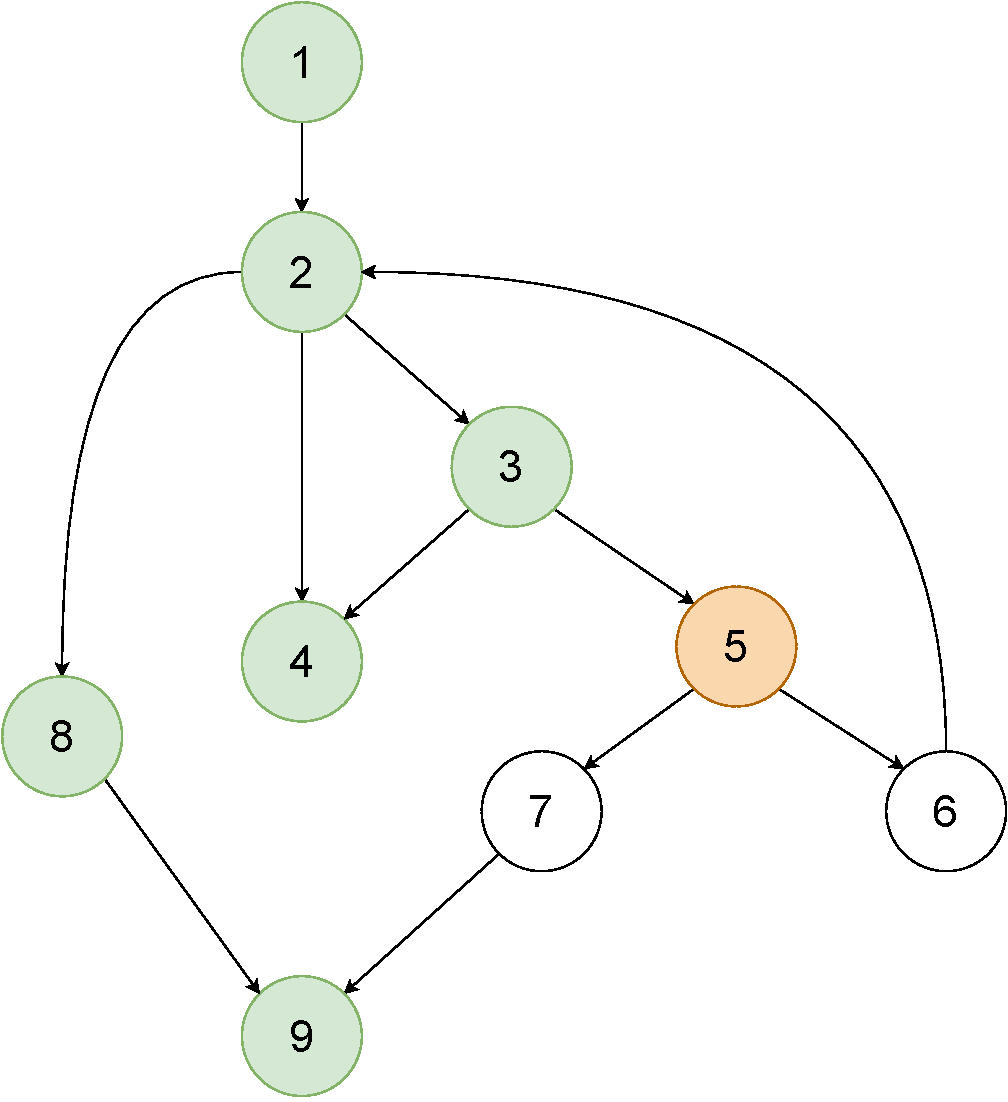
\includegraphics[width=0.3\linewidth]{figures/ad/AD_Path_Prio_CFG.pdf}
    \caption{Control flow graph example for path prioritization}
    \label{fig:cfg_pathprioritization}
\end{figure}

In the sample control flow graph in Figure~\ref{fig:cfg_pathprioritization}, assuming that all branches are symbolic, and the green nodes have been explored, once the two branches from node 3 are identified, the exploration of the branch towards node 5 receives the maximum priority of 100, as it has never been explored before. 
Moreover, immediate children of node 5 also inherit 20\% of the priority of their parent (i.e., 20) as they are the descendants of a newly discovered node. 

We store the reanimation logs on a priority queue, and as a result, workers will explore branches with a higher score first. 
We will compare and contrast the performance of DFS vs. Branch coverage path prioritization methods in Section~\ref{sec:path_priority}. 

\subsection{Debloating the Web Applications}
\animatedead{} produces the code-coverage information by merging the individual code-coverage from each execution of its workers. 
These results are analogous to the dynamic code-coverage used for debloating by the prior work. 
% The main benefit of this approach is the ability to perform an offline analysis based on web server logs.  
After generating the code-coverage for each web application, \animatedead{}'s debloating engine (Step 5 in Figure~\ref{fig:ad_diagram}) performs a reachability analysis and removes unused modules (i.e., files and functions) from the source code of web applications. 
We report the size reduction and security gains of debloating web applications via concolic execution and contrast the performance of this debloating scheme with the dynamic debloating of Less is More in Section~\ref{sec:results}. 

\subsection{Correctness Tests During Development}

During the initial stages of the development of our emulator, we started extracting the list of all PHP instructions from the PHP parser and provided an implementation of their logic in our emulator. 
Next, we analyzed the source code of popular PHP applications such as WordPress and phpMyAdmin to extract samples of interactions with symbolic variables (i.e., database queries, code handling HTTP requests, etc.).  

\paragraph{Unit Tests:} Based on the code snippets extracted from these applications, we created a total of 199 unit tests. 
We also included 19 unit tests provided by MalMax in our test suite~\cite{naderi2019malmax}. 

\paragraph{Functional Tests:} To complement the unit tests, we ran the Selenium scripts published as part of ``Less is More''~\cite{azad2019less} on debloated web applications. 
For the web applications in our dataset that are not part of LIM's dataset, we assembled a list of tasks exercising the main functionality of these web applications. 
For HotCRP, our scripts automate the setup of a conference and its deadline, user creation, submission of papers, and submitting reviews. 
For FluxBB, we automate user creation, posting new topics and changing user preferences. 
The extensive list of tasks that we automated with Selenium scripts is available in the Appendix. 

We then compared the list of invoked files and functions in response to requests towards debloated web applications and through iterative debugging we identified and addressed the implementation bugs that would prevent \animatedead{} from invoking the same modules as listed in the dynamic code-coverage traces. 